\subsection{UC6 - Creazione riunione su piattaforma esterna}
\begin{itemize}
    \item \textbf{Identificativo}: UC6
    \item \textbf{Nome}: Creazione riunione su piattaforma esterna
    \item \textbf{Descrizione grafica}:
\end{itemize}
\begin{center}
    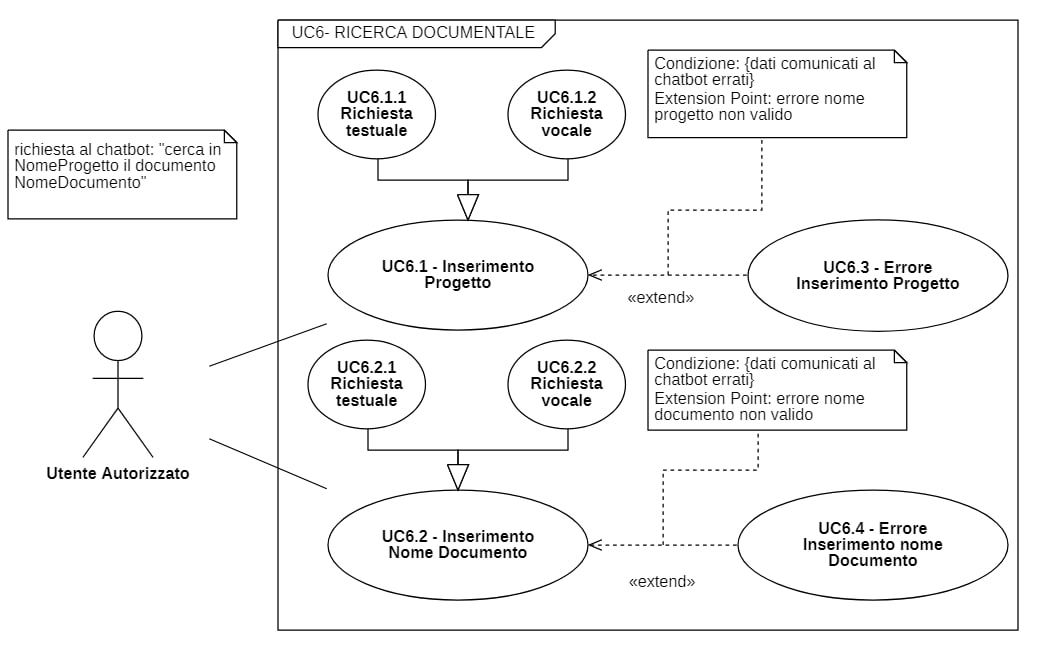
\includegraphics{images/UC6.png} 
\end{center}
 \begin{itemize}
    \item \textbf{Attori}
 \begin{itemize} 
    \item \textit{Primari}: utente autorizzato e loggato sulla piattaforma per videoconferenze
    \item \textit{Secondari}: non presenti
 \end{itemize}
 \item \textbf{Precondizione}: l'utente è autorizzato e loggato sulla piattaforma esterna per videoconferenze desiderata, e si trova nell'interfaccia del chatbot.
 \item \textbf{Postcondizione}: il chatbot risponde alla richiesta dell'utente e invia la richiesta per la creazione della riunione.
 \item \textbf{Scenario principale}: l'utente autorizzato e loggato sulla piattaforma per videoconferenze richiede la creazione di una riunione, specificando la piattaforma (UC6.1), la data (UC6.2) e l'ora (UC6.3) desiderati e la lista dei partecipanti (UC6.4).
 \item \textbf{Estensioni}: 
 \begin{itemize} 
    \item il chatbot comunica all'utente che l'azione non è andata a buon fine (UC10).
    \item il chatbot comunica all'utente che non è stato in grado di interpretare il comando (UC2).
    \item il chatbot comunica all'utente che uno o più parametri specificati non sono corretti (UC6.5 UC6.6 UC6.7 UC6.8).
 \end{itemize}
\end{itemize}
\newpage
\subsubsection{UC6.1 - Inserimento piattaforma per videoconferenze}
\begin{itemize}
    \item \textbf{Identificativo}: UC6.1
    \item \textbf{Nome}: inserimento piattaforma per videoconferenze
    \item \textbf{Descrizione grafica}: (approfondita in UC6)
    \item \textbf{Attori}
 \begin{itemize} 
    \item \textit{Primari}: utente autorizzato e loggato sulla piattaforma per videoconferenze
    \item \textit{Secondari}: non presenti
 \end{itemize}
 \item \textbf{Precondizione}: l'utente comunica al chatbot la richiesta di creazione di una riunione.
 \item \textbf{Postcondizione}: l'utente ha comunicato al chatbot la piattaforma sulla quale verrà creata la riunione.
 \item \textbf{Scenario principale}: il chatbot chiede all'utente su quale applicazione desidera creare la riunione. L'utente comunica al chatbot la piattaforma tramite messaggio testuale (UC6.1.1) o vocale (UC6.1.2).
 \item \textbf{Estensioni}: 
 \begin{itemize} 
    \item il chatbot comunica all'utente che la piattaforma per videoconferenze inserita non è corretta (UC6.5).
 \end{itemize}
\end{itemize}
\subsubsection{UC6.2 - Inserimento data per la riunione}
\begin{itemize}
    \item \textbf{Identificativo}: UC6.2
    \item \textbf{Nome}: inserimento data per la riunione
    \item \textbf{Descrizione grafica}: (approfondita in UC6)
    \item \textbf{Attori}
 \begin{itemize} 
    \item \textit{Primari}: utente autorizzato e loggato sulla piattaforma per videoconferenze
    \item \textit{Secondari}: non presenti
 \end{itemize}
 \item \textbf{Precondizione}: l'utente comunica al chatbot la richiesta di creazione di una riunione.
 \item \textbf{Postcondizione}: l'utente ha comunicato al chatbot la data alla quale verrà creata la riunione.
 \item \textbf{Scenario principale}: il chatbot chiede all'utente in che data desidera creare la riunione. L'utente comunica al chatbot la data tramite messaggio testuale (UC6.1.1) o vocale (UC6.1.2).
 \item \textbf{Estensioni}: 
 \begin{itemize} 
    \item il chatbot comunica all'utente che la data inserita non è corretta, oppure risulta indisponibile (UC6.6).
 \end{itemize}
\end{itemize}
\subsubsection{UC6.3 - Inserimento ora per la riunione}
\begin{itemize}
    \item \textbf{Identificativo}: UC6.3
    \item \textbf{Nome}: inserimento ora per la riunione
    \item \textbf{Descrizione grafica}: (approfondita in UC6)
    \item \textbf{Attori}
 \begin{itemize} 
    \item \textit{Primari}: utente autorizzato e loggato sulla piattaforma per videoconferenze
    \item \textit{Secondari}: non presenti
 \end{itemize}
 \item \textbf{Precondizione}: l'utente comunica al chatbot la richiesta di creazione di una riunione.
 \item \textbf{Postcondizione}: l'utente ha comunicato al chatbot l'ora alla quale verrà creata la riunione.
 \item \textbf{Scenario principale}: il chatbot chiede all'utente a che ora desidera creare la riunione. L'utente comunica al chatbot l'ora tramite messaggio testuale (UC6.1.1) o vocale (UC6.1.2).
 \item \textbf{Estensioni}: 
 \begin{itemize} 
    \item il chatbot comunica all'utente che l'ora inserita non è corretta, oppure risulta indisponibile (UC6.7).
 \end{itemize}
\end{itemize}
\subsubsection{UC6.4 - Inserimento partecipanti}
\begin{itemize}
    \item \textbf{Identificativo}: UC6.4
    \item \textbf{Nome}: inserimento partecipanti
    \item \textbf{Descrizione grafica}: (approfondita in UC6)
    \item \textbf{Attori}
 \begin{itemize} 
    \item \textit{Primari}: utente autorizzato e loggato sulla piattaforma per videoconferenze
    \item \textit{Secondari}: non presenti
 \end{itemize}
 \item \textbf{Precondizione}: l'utente comunica al chatbot la richiesta di creazione di una riunione.
 \item \textbf{Postcondizione}: l'utente ha comunicato al chatbot i partecipanti alla riunione che verrà creata.
 \item \textbf{Scenario principale}: il chatbot chiede all'utente quali sono i partecipanti alla riunione. L'utente comunica al chatbot i partecipanti tramite messaggio testuale (UC6.1.1) o vocale (UC6.1.2).
 \item \textbf{Estensioni}: 
 \begin{itemize} 
    \item il chatbot comunica all'utente che uno o più partecipanti non sono stati inseriti in modo corretto (UC6.8).
 \end{itemize}
\end{itemize}
\subsubsection{UC6.5 - Errore inserimento piattaforma per videoconferenze}
\begin{itemize}
    \item \textbf{Identificativo}: UC6.5
    \item \textbf{Nome}: errore inserimento piattaforma per videoconferenze
    \item \textbf{Descrizione grafica}: (approfondita in UC6)
    \item \textbf{Attori}
 \begin{itemize} 
    \item \textit{Primari}: utente autorizzato e loggato sulla piattaforma per videoconferenze
    \item \textit{Secondari}: non presenti
 \end{itemize}
 \item \textbf{Precondizione}: l'utente ha inserito una piattaforma per videoconferenze non valida o non supportata.
 \item \textbf{Postcondizione}: il chatbot comunica all'utente che la piattaforma inserita non è valida.
 \item \textbf{Scenario principale}: il chatbot comunica all'utente l'errore nell'inserimento della piattaforma esterna per videoconferenze e chiede di reinserirla.
\end{itemize}
\subsubsection{UC6.6 - Errore inserimento data per la riunione}
\begin{itemize}
    \item \textbf{Identificativo}: UC6.6
    \item \textbf{Nome}: errore inserimento data per la riunione
    \item \textbf{Descrizione grafica}: (approfondita in UC6)
    \item \textbf{Attori}
 \begin{itemize} 
    \item \textit{Primari}: utente autorizzato e loggato sulla piattaforma per videoconferenze
    \item \textit{Secondari}: non presenti
 \end{itemize}
 \item \textbf{Precondizione}: l'utente ha inserito una data non valida o indisponibile.
 \item \textbf{Postcondizione}: il chatbot comunica all'utente che la data inserita non è valida o è indisponibile.
 \item \textbf{Scenario principale}: il chatbot comunica all'utente l'errore nell'inserimento della data e chiede di reinserirla.
\end{itemize}
\subsubsection{UC6.7 - Errore inserimento ora per la riunione}
\begin{itemize}
    \item \textbf{Identificativo}: UC6.7
    \item \textbf{Nome}: errore inserimento ora per la riunione
    \item \textbf{Descrizione grafica}: (approfondita in UC6)
    \item \textbf{Attori}
 \begin{itemize} 
    \item \textit{Primari}: utente autorizzato e loggato sulla piattaforma per videoconferenze
    \item \textit{Secondari}: non presenti
 \end{itemize}
 \item \textbf{Precondizione}: l'utente ha inserito un'ora non valida o indisponibile.
 \item \textbf{Postcondizione}: il chatbot comunica all'utente che l'ora inserita non è valida o è indisponibile.
 \item \textbf{Scenario principale}: il chatbot comunica all'utente l'errore nell'inserimento dell'ora e chiede di reinserirla.
\end{itemize}
\subsubsection{UC6.8 - Errore inserimento partecipanti}
\begin{itemize}
    \item \textbf{Identificativo}: UC6.8
    \item \textbf{Nome}: errore inserimento partecipanti
    \item \textbf{Descrizione grafica}: (approfondita in UC6)
    \item \textbf{Attori}
 \begin{itemize} 
    \item \textit{Primari}: utente autorizzato e loggato sulla piattaforma per videoconferenze
    \item \textit{Secondari}: non presenti
 \end{itemize}
 \item \textbf{Precondizione}: l'utente ha inserito uno o più partecipanti in modo non corretto.
 \item \textbf{Postcondizione}: il chatbot comunica all'utente che uno o più partecipanti sono stati inseriti in modo non corretto.
 \item \textbf{Scenario principale}: il chatbot comunica all'utente l'errore nell'inserimento dei partecipanti e chiede di reinserirli.
\end{itemize}
\newpage